\documentclass[a4paper]{article}

\usepackage[utf8]{inputenc}
\usepackage[serbian]{babel}

\usepackage{tikz}
\usepackage{tcolorbox}
\usepackage{amsmath}
\usepackage{amsthm}
\usepackage{float}
\usepackage{listings}
\usepackage{fancyhdr}

\begin{document}
    \begin{titlepage}
    \begin{tabular}{ l  c   r  }
        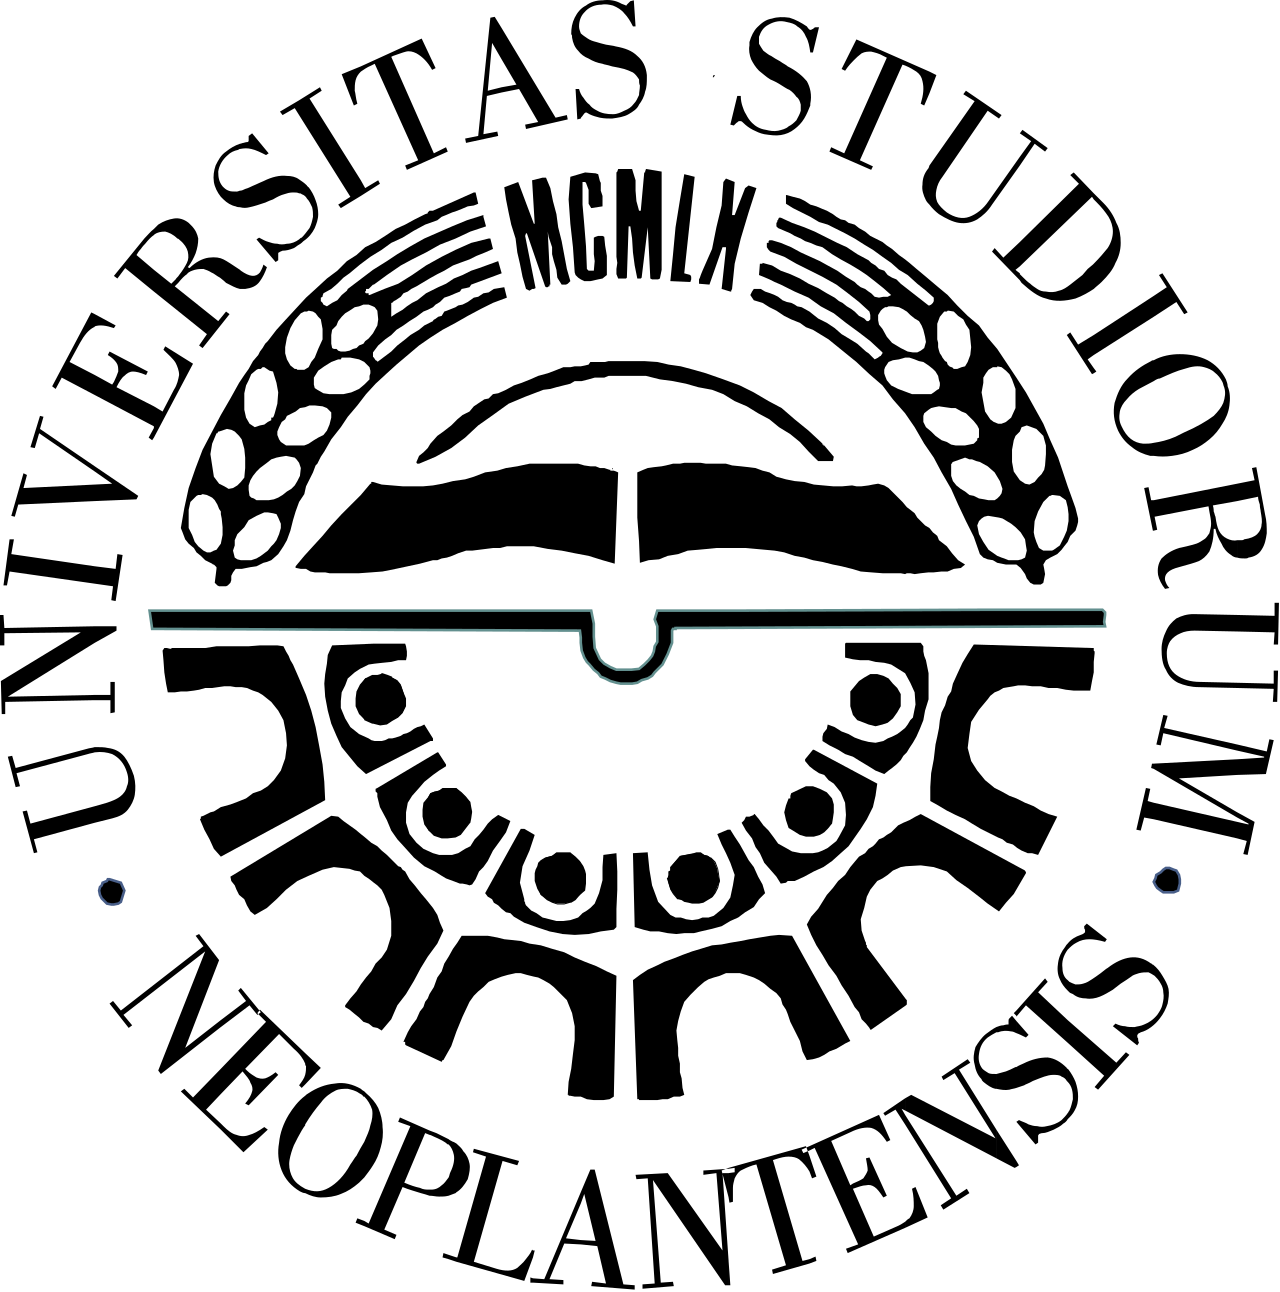
\includegraphics[height=0.1\textwidth, width=0.1\textwidth]{img/uns.png} &
        \begin{tabular}{c}
            \large\textbf{UNIVERZITET U NOVOM SADU} \\
            \large\textbf{FAKULTET TEHNIČKIH NAUKA}  \\
        \end{tabular}
        
\includegraphics[height=0.1\textwidth, width=0.1\textwidth]{img/ftn-logo.jpg}
    \end{tabular}
    \vspace*{1cm}
    \begin{flushleft}
        UNIVERZITET U NOVOM SADU \\
        FAKULTET TEHNIČKIH NAUKA \\
        NOVI SAD \\
        Departman za računarstvo i automatiku \\
        Odsek za računarsku tehniku i računarske komunikacije \\
    \end{flushleft}
    \vspace*{2cm}
    \begin{center}
        \LARGE\textbf{ISPITNI RAD}
    \end{center}
    \vspace*{0.25cm}
    \begin{flushleft}
        \begin{tabular}{l l}
            Kandidat:& Lazar Nagulov \\
            Broj indeksa:& SV61/2022 \\
            & \\
            Predmet:&    Objektno orijentisano programiranje 2 \\
            Tema rada:&	Sudoku \\
            & \\
            & \\
            Mentor rada:&    dr Miodrag Đukić
        \end{tabular}
    \end{flushleft}
    \vfill
    \begin{center}
        Novi Sad, decembar, 2023.
    \end{center}
\end{titlepage}
    \pagestyle{fancy}
    
\rhead{SADRŽAJ}
\lhead{}
\pagenumbering{Roman}
\tableofcontents
\newpage

\rhead{SPISAK SLIKA}
\listoffigures
\newpage

\rhead{SPISAK TABELA}
\listoftables
\newpage
    
    \section{Uvod}
    \pagenumbering{arabic}
    \rhead{1. Uvod}
    \subsection{Sudoku}
    Sudoku je logička zagonetka najčešće u obliku $9 \times 9$ tabele (matrice).
    U prazna polja tabele se upisuju cifre, tako da se svaka broj mora pojaviti
    tačno jednom u svakom redu, svakoj koloni i svakoj $3\times 3$ podmatrici (bloku).
    \begin{figure}[h]
        \centering
        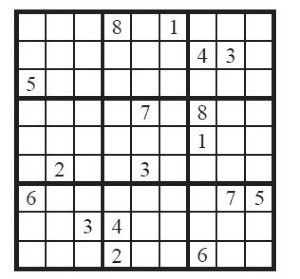
\includegraphics[width=0.5\textwidth, height=0.5\textwidth]{img/sudoku-example.jpg}
        \caption{Primer sudoku zagonetke}
    \end{figure}
    \par Zagonetka ne mora da ima jedno rešenje, ali je standard da ga ima. Primer rešenje zagonetke sa slike 1:
    \begin{figure}[h]
        \centering
        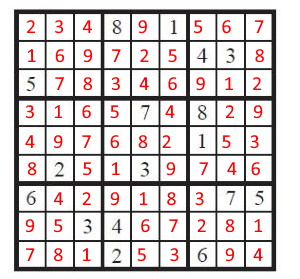
\includegraphics[width=0.5\textwidth, height=0.5\textwidth]{img/sudoku-example-sol.jpg}
        \caption{Primer rešenja sudoku zagonetke}
    \end{figure}
    \subsection{Zadatak}
    Realizovati konzolnu aplikaciju koja omogućava rešavanje i generisanje sudoku zagonetki. Korisnik unosi dateteke kroz argumente komandne linije. 
    Primer pokretanja programa:
    \par\texttt{./sudoku $input.txt$ $output.txt$}\\
    Argumenti:
    \begin{enumerate}
        \item $input.txt$ - Datoteka iz koje se čita zagonetka.
        \item $output.txt$ - Datoteka u koju se upisuje zagonetka.
    \end{enumerate}
    \par Svaka datoteka sadrži \texttt{jednu} zagonetku, svaki red predstavlja jedan red u tabeli, i svako polje je odvojeno razmakom. Ukoliko datoteke nisu navedene,
    korisniku se ispisuje način korišćenja programa.
    \par Nakon uspešnog pokretanja programa, prikazuje se početni meni koji nudi opcije:
    \begin{itemize}
        \item \texttt{Generate new Sudoku puzzle} - Generisanja nove zagonetke.
        \item \texttt{Load Sudoku puzzle from file} - Učitavanja zagonetke.
        \item \texttt{Exit} - Izlaska iz igre.
    \end{itemize}
    Generisana zagonetka se upisuje u $output.txt$ datoteku.
    Nakon generisanja ili učitavanja zagonetke, korisnik može da:
    \begin{itemize}
        \item \texttt{Import solution} - Učita rešenje.
        \item \texttt{Solve} - Dopusti programu da reši zagonetku.
        \item \texttt{Exit} - Izlađe iz igre.
    \end{itemize}
    \par Na konzolnoj aplikaciji, posle rešenja koje je generisao program ili učitao iz datoteke, prikazuju se statistički podaci igre, uključujući broj dobro 
    postavljenih polja, broj grešaka i brojač odigranih igara i spisak svih pronađenih grešaka. Nakon završetka igre, korisnik ima opciju da odabere ponovno igranje, 
    što pokreće novu iteraciju igre.
    \newpage

    \rhead{2. Analiza problema}
    \section{Analiza problema}
    \par Glavni problem zadatka je mogućnost rešavanja zagonetke, jer nam je algoritam za rešavanju zagonetke neophodan za generisanje iste.
    Najčešći način koji se koristi u rešavanju zagonetke je isprobavajući svaka moguća rešenja. Sam algoritam je rekurzivan, što može da dovede do 
    prelivanja steka (eng. Stack overflow), što znači da moramo da umanjivo broj mogućih rekurzivnih poziva.
    \par Pozitivna strana ovoga algoritma koji pokušava sve mogućnosti je sigurno pronalaženje rešenja za svaku zagonetku (ukoliko ono postoji) i što u osnovi ne koristi dodatne strukture podataka izuzev same tabele.
    Nažalost, za uveđenje optimizacije neophodno je zauzeti veći deo memorije za pomoćne strukture, poput haš tabele ukoliko želimo da ubacimo heruistiku - praćenje pojavljivanje brojeva, ili niz bitova
    ukoliko želimo da brzo proverimo da li je moguće postaviti broj u određeno polje. Primetimo da prethodne ideje za optimizaciju zahtevaju prolazak kroz čitavu tabelu pre samog algoritma za rešavanje,
    što može biti skupo za jednostavne zagonetke.
    \par Za potrebe projekta, uvedena je optimizacija koja ubrzava proveru da li je moguće postaviti broj u dato polje. Ideje za dalju optimizaciju su ovođene prethodno navedene heruistike ili
    korišćene nekih od probalističkih algoritama, poput Knutovog algoritma (eng. Knuth's Algorithm). 
    \par Takođe moramo razmotriti mogućnosti generisanje pseudoslučajnih brojeva za generisanje tabele. Primećujemo da korišćenjem obične random funkcije često generiše iste,
    ili veoma slične tabele.
    \newpage

    \rhead{3. Koncept rešenja}
    \section{Koncept rešenja}
    
    \subsection{Algoritmi za rešavanje zagonetke}
    \subsubsection{Obrnuta pretraga}
    Najčešće korišćen algoritam za rešavanje sudoku zagonetke je obrnuta pretraga (eng. Backtracking).
    Ovo je algoritam grube sile (eng. Brute force) koji isprobava sve moguće kombinacije. Dakle, potrebno je da se prođe kroz
    svako polje u tabeli. Ukoliko je polje prazno, upisujemo cifru koja u trenutnoj tabeli ispunjava sva pravila. Nakon upisivanje cifre, rekurzivno pozivamo funkciju 
    - pokušavamo da pronađe rešenje sa novom tabelom. Ukoliko rešenje nije pronađeno, vraćamo se nazad i upisujemo drugu cifru. 
    \par Vremenska složenost ovog algoritma je $\mathcal{O}(n ^ m)$, gde je $n$ dimenzija tabele, a $m$ broj polja koja trebaju da se popune.
    (U našem slučaju je složenost $\mathcal{O}(9^n)$). Minimalan broj polja koja
    moraju biti popunjena je $17$, dakle, u najgorem slučaju se provera $9^{64}$ mogućnosti!
    
    \subsubsection{Optimizacija obrnute pretrage}
    Način na koji možemo optimizovati algoritam obrnute pretrage je da ubrzamo proveru da li se broj može postaviti na zadatoj poziciji. To ćemo postići tako što ćemo pamtiti
    koji broj se našao u redu, koloni i bloku. Za to ćemo koristiti \texttt{std::bitset} iz zaglavlja \texttt{bitset} gde, ako se za $i \in [0,8]$ na $i$-toj poziciji nalazi 1, znači da se cifra $i+1$ nalazi u redu, koloni ili bloku.
    \par Pre samog ulaska u rekurzivnu funkciju obrnute pretrage, moramo proći kroz tabelu i zapisati svaki broj koji se nalazi u tabeli u nizove bitova. Potrebna su 3 niza bitova - 
    \begin{figure}[h]
        \centering
        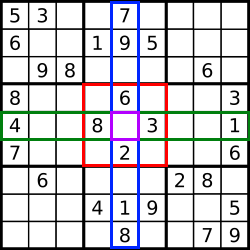
\includegraphics[width=0.5\textwidth, height=0.5\textwidth]{img/conversion.png}\\
        \texttt{Polje (4,4)}\\
        \begin{tabular}{ l r }
            \texttt{RowSet: } & \texttt{010001101}\\
            \texttt{ColSet: } & \texttt{111100011}\\
            \texttt{BlockSet:}& \texttt{010100110}\\
        \end{tabular}
        \caption{Primer konverzije polja u binaran broj}
    \end{figure}
    za red, kolonu i blok. Za proveru da li je cifru moguće upisati
    koristimo bitnu operaciju ili (eng. bitwise or): 
    \par\texttt{std::bitset<> contain = rows[row] | cols[col] | blocks[block];}\\
    Novi niz bitova \texttt{contain} ima $0$ na $i$-toj poziciji ako je moguće postaviti cifru $i+1$ na poziciju '(row, col)'. Na slici 3 vidimo da se u 
    redu nalaze brojevi 1,3,4,8 (010001101), koloni 7,9,6,2,1,8 (111100011) i u bloku 6,3,2,8 (010100110). Iz ovoga zaključujemo da je u polje (4,4)
    moguće upisati broj 5 (111101111).
    \par Vremenska složenost je i dalje $\mathcal{O}(n^m)$, gde je $n$ dimenzija tabele, a $m$ broj polja koja trebaju da se popune, stim da je su sve provere da li se broj može upisati 
    u polje svedene na $\mathcal{O}(m)$ za razliku od prethodnog algoritma koji ima složenost $\mathcal{O}(nm)$. 
    \par U Tabeli 1. vidimo da se prosečno vreme rešavanja duplo brže. Sam test je sproveden na 1000 tabela koja sadrže 25 popunjenih polja.
    \begin{table}[h]
        \centering
        \begin{tabular}{ |c|c|c|c|}
            \hline
            & Maksimum & Medijana & Srednja vrednost \\
            \hline
            Gruba sila & 6.20147s & 0.001222s & 0.04691s \\
            \hline
            Optimizacija & 2.14567s & 0.00072s & 0.02301s \\
            \hline
        \end{tabular}
        \caption{Optimizacija obrnute pretrage}
    \end{table}

    \subsection{Algoritmi za generisanje zagonetke}
    \begin{figure}[H]
        \centering
        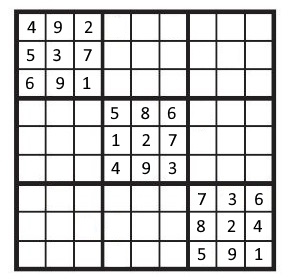
\includegraphics[width=0.25\textwidth, height=0.25\textwidth]{img/diag-fill.jpg}
        $\longrightarrow$
        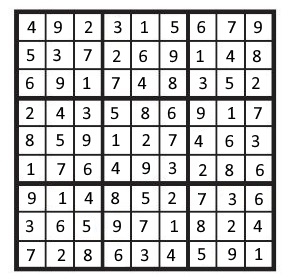
\includegraphics[width=0.25\textwidth, height=0.25\textwidth]{img/full.jpg}
        $\longrightarrow$
        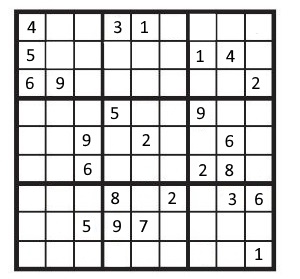
\includegraphics[width=0.25\textwidth, height=0.25\textwidth]{img/generated.jpg}
        \caption{Primer generisanje zagonetke}
    \end{figure}
    \subsubsection{Koraci u generisanju zagonetke}
    Generisanje zagonetke se može opisati u dva koraka:
    \begin{enumerate}
        \item Popuniti čitavu tabelu slučajnim vrednostima [1, \texttt{BOARD\_SIZE}].
        \item Nasumično obrisati brojeve iz tabele.
    \end{enumerate}
    
    \par Primetimo da se blokovi na glavnoj dijagonali mogu zasebno popuniti jer ne utiču jedan na drugog. Dakle, prvi korak u generisanju se svodi na 
    popunjavanja glavne dijagonale i rešavanja tako generisane zagonetke. Zatim brišemo brojeve iz tabele. Koliko brojava trebamo obrisati zavisi od težine zagonetke
    koju želimo generisati (Tabela 2).
    \begin{table}[H]
        \centering
        \begin{tabular}{ | c | c |}
            \hline
            Težina & Broj popunjenih polja \\
            \hline
            Lako & 32 - 38\\
            \hline
            Srednje & 26 - 31\\
            \hline
            Teško & 22 - 25\\
            \hline
            Veoma teško & 17 - 21\\
            \hline
        \end{tabular}
        \caption{Težina zagonetke u odnosu na broj popunjenih polja}
    \end{table}
    \subsubsection{Generisanje pseudoslučajnih brojeva}
    Za generisanje pseudoslučajnih brojeva koristimo Mersen Tviser algoritam (eng. Mersenne Twister algorithm). 
    Implementacija samog algoritma se nalazi u zaglavlju \texttt{random} (\texttt{std::mt19937}). Algoritam ima ogroman period ($2^{19937}-1$), što znači da se niz
    brojeva neće ponavljati. Seme (eng. seed) se nasumično određujemo koristeći \texttt{std::random\_device}, a za samo generisanje brojeva u određenom intervalu
    koristimo \texttt{std::uniform\_int\_distribution}.
    \par Ovo nam omogućava generisanje nasumičnih brojeva visokog kvaliteta.
    \subsection{Algoritmi za proveru validnosti zagonetke}


    \newpage
    \rhead{4. Opis rešenja}
    \section{Opis rešenja}
    
    \subsection{Modul glavnog programa (Main)}
    \subsubsection{Funkcija main}
    \texttt{int main(int argc, char** argv);}
    \par Glavna funckija programa. Kreira objekat tipa Sudoku i prosleđuje mu imena datoteka prosleđenih preko argumenata komandne linije.
    \subsubsection{Funkcija za pomoć prilikom pokretanja (Usage)}
    \texttt{void Usage();}
    \par Ispisuje način pokretanja programa u slučaju da potrebni parametri nisu navedeni.

    \subsection{Modul Sudoku (Sudoku)}
    Glavni modul koji povezuje sve funkcionlanosti iz modula tabele u jednu celinu.
    \subsubsection{Članovi}
    \begin{tabular}{ l l }
        \texttt{std::string inputFile} & Naziv ulazne datoteke\\
        \texttt{std::string outputFile} & Naziv izlazna datoteke\\
        \texttt{int currentRound;} & Trenutna runda\\
        \texttt{int correctCount;} & Broj tačnih cifara\\
        \texttt{int wrongCount;} & Broj pogrešnih cifara\\
        \texttt{Board board;} & Sudoku tabela\\
    \end{tabular}
    
    \subsubsection{Enumeracije}
    \texttt{enum Difficulty;}
    \par Određuje težinu Sudoku zagonetke na osnovu broja izbrisanih polja. \\ 
    Vrednost: \texttt{EASY, MEDIUM, HARD, VERY\_HARD}

    \subsubsection{Konstruktor}
    \texttt{Sudoku(std::string\& inputFile, std::string\& outputFile)}
    \par Glavni parametrizovani kontstruktor.\\
    Parametri:
    \begin{itemize}
        \item (\texttt{std::string\&}) inputFile - ime datoteke iz koje će se čitati zagonetka ili njeno rešenje.
        \item (\texttt{std::string\&}) outputFile - ime datoteke u koju će se upisivati rešenje ili novo generisana zagonetka.
    \end{itemize}

    \subsubsection{Funkcija članica za pokretanje (Run)}
    \texttt{void Run();}
    \par Pokreće aplikaciju i kreira početni meni za korisnika. Nudi korisniku mogu\-ćnost da generiše 
    ili učita zagonetku iz datoteke. Nakon generisanja ili učitavanja zagonetke, korisnik može da izabere način rešavanja.

    \subsubsection{Funcija članica za unos rešenja (SolvingOptions)}
    \texttt{void SolvingOptions();}
    \par Nudi korisniku mogućnost da učita rešenje ili da dopusti programu da sam reši zagonetku. Poziva se  iz \texttt{Run()} funkcije nakon generisanja 
    ili učitavanja zagonetke.

    \subsubsection{Funkcija članica za rešavanje zagonetke (Solve)}
    \texttt{void Solve();}
    \par Rešava zagonetku koristeći algoritam obrnute pretrage. Rešenje upisuje u $output.txt$ datoteku prosleđenu preko argumentana komandne linije.

    \subsubsection{Funckija članica za proveru rešenja (CheckSolution)}
    \texttt{void CheckSolution();}
    \par Učitava zagonetku iz $input.txt$ datoteke prosleđene preko argumentana komandne linije i proverava koliko ima grešaka. Ispisuje sve greške koje pronađe, njihov broj i broj tačno upisanih brojeva.

    \subsubsection{Funkcija članica za gerenisanje zagonetke (Generate)}
    \text{void Generate(Difficulty difficulty);}
    \par Generiše Sudoku zagonetku sa zadatom težinom. Upisuje generisanu tabelu u $output.txt$ datoteku prosleđenu preko argumentana komandne linije.\\
    Parametri:
    \begin{itemize}
        \item (\texttt{Sudoku::Difficulty}) difficulty - enumeracija koja označava težinu zagonetke.
    \end{itemize}
   
    \subsection{Modul Tabela (Board)}
    Modul koji sadrži pomoćne funkcije potrebne za menjanje trenutne tabele ili provere njene validnosti.
    \subsubsection{Konstante}
    \begin{tabular}{ l l }
        \par\texttt{int BOARD\_SIZE = 9;} & Veličina tabele. \\
        \par\texttt{int BLOCK\_SIZE = 3;} & Veličina bloka. \\
        \par\texttt{int EMPTY = 0;}  & Oznaka za prazno polje. \\
        \par\texttt{char EMPTY\_CHAR = '\_';}  & Oznaka za prazno polje prilikom ispisa.
    \end{tabular}
    
    \subsubsection{Članovi}
    \begin{tabular}{ l l }
        \par\texttt{int board[BOARD\_SIZE * BOARD\_SIZE];} & Niz koji predstavlja tabelu.\\
    \end{tabular}

    \subsubsection{Alijas BitArray}
    {\parindent0pt
    \texttt{using BitArray = }\\
    \texttt{std::array<std::bitset<Board::BOARD\_SIZE>, Board::BOARD\_SIZE>;}
    }
    \par Niz od \texttt{Board::BOARD\_SIZE} setova bitova dužine \texttt{Board::BOARD\_SIZE}.
    
    \subsubsection{Funkcija članica za proveru poteza (IsPossibleMove)}
    \texttt{bool IsPossibleMove(int row, int col, int number) const;}
    \par Proverava da li postavka datog broja na datu poziciju je validan potez.
    Parametri:
    \begin{itemize}
        \item (\texttt{int}) row - red u tabeli
        \item (\texttt{int}) col - kolona u tabeli
        \item (\texttt{int}) number - broj koji se pokušava staviti
    \end{itemize}
    Povratna vrednost:
    \begin{itemize}
        \item (\texttt{bool}) - true ako je moguće postaviti broj, false ako nije.
    \end{itemize}

    \subsubsection{Funckija članica za proveru validnosti tabele (IsValid)}
    \texttt{bool IsValid() const;}
    \par Proverava da li trenutna tabela ispunjava sva pravila sudoka.
    Povratna vrednost:
    \begin{itemize}
        \item (\texttt{bool}) True ako je trenutna tabela validna.
    \end{itemize}

    \subsubsection{Funkcija članica za pronalaženje grešaka (CountErrors)}
    \texttt{int CountErrors(const Board\& original) const;}
    \par Prebrojava i ispisuje sve greške u tabeli.\\
    Parametri:
    \begin{itemize}
        \item (\texttt{const Board\&}) original - Originalna tabela pre rešavanja.
    \end{itemize}
    Povratna vrednost:
    \begin{itemize}
        \item (\texttt{int}) Broj grešaka u tabeli.
    \end{itemize}

    \subsubsection{Funkcija članica za dobavljanje elementa tabele (At)}
    \texttt{int\& At(int row, int col);}
    \par\texttt{const int\& At(int row, int col) const;}
    \par Dobavlja element na poziciji '(row, col)'. Proverava granice. Baca \\ \texttt{std::out\_of\_range} u slučaju da
    su uneti brojevi nevalidni.
    
    \subsubsection{Statična funkcija članica za dobavljanja blocka (GetBlock)}
    \texttt{static inline int GetBlock(int row, int col);}
    \par Vraća blok u kome se nalazi polje '(row, col)'.\\
    Parametri:
    \begin{itemize}
        \item (\texttt{int}) row - Red u tabeli.
        \item (\texttt{int}) col - Kolona u tabeli.
    \end{itemize}
    Povratna vrednost:
    \begin{itemize}
        \item (\texttt{int}) Broj bloka u kome se nalazi polje (row, col)
    \end{itemize}

    \subsubsection{Funkcija članica za generisanje elemenata na glavnoj dijagonali (GenerateDiagonal)}
	\texttt{void GenerateDiagonal();}
	\par Generiše nasumično elemente na glavnoj dijagonali.

    \subsubsection{Funcija članica za generisanje ostalih elemenata (GenerateOther)}
    \texttt{bool GenerateOther(int row, int col);}
    \par Rekurzivno generiše nasumično elemente koji se ne nalaze na glavnoj dijagonali.\\
	Parametri:
    \begin{itemize}
        \item (\texttt{int}) row - Početan red (uglavnom 0).
        \item (\texttt{int}) col - Početna kolona (uglavnom 0).
    \end{itemize}
    Povratna vrednost:
    \begin{itemize}
        \item (\texttt{bool}) Zaustavlja rekurzivno generisanje tabele.
    \end{itemize}
    
    \subsubsection{Funkcija članica za popunjavanje blokova (FillBlock)}
    \texttt{void FillBlock(int row, int col);}
    \par Rekurzivno generiše nasumično elemente u bloku.\\
    Parametri:
    \begin{itemize}
        \item (\texttt{int}) row - početni red (gornje levo polje u bloku).
        \item (\texttt{int}) col - početna kolona (gornje levo polje u bloku).
    \end{itemize}

    \subsubsection{Funkcija članica za brisanje elemenata iz tabele (RemoveNumber)}
	\texttt{void RemoveNumber(int count);}
    \par Nasumično briše $count$ elementa iz tabele.\\
    Parametri:
    \begin{itemize}
        \item (\texttt{int}) count - broj elemenate koliko se briše iz tabele.
    \end{itemize}

    \subsubsection{Funkcija članica koja implementira algoritam obrnute pretrage (Backtrack)}
    {\parindent0pt
    \texttt{bool Backtrack(BitArray\& rSet, BitArray\& cSet, BitArray\& bSet);}
    }
    \par Funkcija implementira algoritam obrnute pretrage. Rekurzivno popunjava tabelu. Poziva se iz funkcije \texttt{Solve()} nakon generisanja pomoćnih nizova bitova.
    Parametri:
    \begin{itemize}
        \item (\texttt{BitArray}) rSet - Pomoćni niz koji prati pojavljivanje brojeva u redovima.
        \item (\texttt{BitArray}) cSet - Pomoćni niz koji prati pojavljivanje brojeva u kolonama.
        \item (\texttt{BitArray}) bSet - Pomoćni niz koji prati pojavljivanje brojeva u blokovima.
    \end{itemize}
    Povratna vrednost:
    \begin{itemize}
        \item (\texttt{bool}) Zaustavlja rekurziju kada pronađe rešenje.
    \end{itemize}

    \subsubsection{Funkcija članica za pronalaženje prvog praznog polja (FindEmpty)}
	\texttt{bool FindEmpty(int\& row, int\& col);}
    \par Pronalazi prvo prazno polje od pozicije '(row, col)'. Prazno polje se nalazi u $row$ i $col$ promenljivi nakon završetka funkcije.\\
    Parametri:
    \begin{itemize}
        \item (\texttt{int\&}) row - referenca na početan red koji se pretražuje.
        \item (\texttt{int\&}) col - referenca na početnu kolonu koja se pretražuje.
    \end{itemize}
    Povratna vrednost:
    \begin{itemize}
        \item True ako postoji prazan element.
    \end{itemize}

    \subsubsection{Funckija članica za brisanje tabele (Clear)}
    \texttt{void Clear();}
    \par Postavlja sve elemente u tabeli na 0.

    \subsubsection{Operatori upisa i ispisa}
    \par\texttt{std::istream\& operator>>(std::istream\& in, Board\& b);}
    \par Operator za čitanje tabele iz datoteke.
    \par\texttt{std::ostream\& operator<<(std::ostream\& out, const Board\& b);}
    \par Operator za ispisivanje tabele na standarni izlaz - konzolu.
    \par\texttt{std::ofstream\& operator<<(std::ofstream\& out, const Board\& b);}
    \par Operator za upisivanje tabele u datoteku. 

    \subsubsection{Operator dobavljanja}
    \par\texttt{int\& operator()(int row, int col);}
    \par\texttt{const int\& operator()(int row, int col) const;}
    \par Operator za dobavljanje elementa na poziciji '(row, col)'.
    
    \newpage
    \rhead{5. Testiranje}
    \section{Testiranje}
    Implementacija se testira pomoću modula \texttt{Test}. Napravljeni su posebni testni skupovi (skupovi testnih slučajeva) za svaki modul, 
    a svaki testni skup sadrži testove (testne slučajeve, test cases) raznih segmenata tog modula - funkcija i struktura, kao i testiranje njihovih međusobnih odnosa.
    \par Testovi se pokreću komandom \texttt{./sudoku -test}.
    \subsection{Testni skupovi}
    {\parindent0pt
        Skup testova za verifikaciju tabele.
        \begin{itemize}
            \item $invalid\_row.txt$
            \item $invalid\_column.txt$
            \item $invalid\_block.txt$
        \end{itemize}
        \par Skup testova za proveru korisnikovog rešenja:
        \begin{itemize}
            \item $original\_changed.txt$ i $error\_changed.txt$
            \item $original\_all.txt$ i $error\_all.txt$
        \end{itemize}    
    }
    \subsection{Testiranje validnosti korisnikove zagonetke (IsValid)}
    
    \subsubsection{Validna zagonetka}
    Test učitava validnu zagonetku.
    \subsubsection{Nevalidna kolona}
    Test učitava zagonetku sa tačno jednim duplikatom u koloni. 
    \subsubsection{Nevalidan red}
    Test učitava zagonetku sa tačno jednim duplikatom u redu.
    \subsubsection{Nevalidan blok}
    Test učitava zagonetku sa tačno jedinim duplikato u bloku.
    
    \subsection{Testiranje provere postavke brojeva (IsPossibleMove)}

    \subsection{Testiranje validnosti korisnikovog rešenja (CountErrors)}
    \subsubsection{Izmena nepraznog početnog polja}
    Test učitava početnu tabelu i rešenu tabelu sa izmenjenim nepraznim poljima. 
    \subsubsection{Sve izmene}
    Test učitava početnu tabelu i rešenu tabelu koja sadrži duplikat u redu, duplikat u koloni, duplikat u bloku i izmenjeno neprazno polje.
    \subsection{Testiranje generisanja tabele (Generate)}

    \subsection{Testiranje rešavanja zagonetke (Solve)}

    \newpage
    \rhead{6. Uočeni problemi i ograničenja}
    \section{Uočeni problemi i ograničenja}
    \newpage
    \rhead{7. Zaključak}
    \section{Zaključak}
    Napravljen je i verifikovan jedan koncept za realizaciju datog problema. Optimizovano je traženje i generisanje rešenje i date su ideje za 
    dodatne optimizacije. 
    \par Rezultati merenja iz Tabele 1 pokazuju znatno ubrzanje, naručito za tabele koje imaju više praznih polja. Ovo je manje primetno za tabele koje imaju 
    manji broj praznih polja, jer je veća verovatnoća da uobičajna pretraga brzo pronađe duplikate. 
    \par Odatle zaključujemo da najviše dobijamo na vremenu kada tabela ima više praznih mesta. Dodatne optimizacije mogu pomoći u tome, ali ni jedna od njih ne 
    garantuje ubrzanje za svaku moguću tabelu, ali zahtevaju dodajno korišćenje memorije.
    \newpage
\end{document}